\chapter{Auditing and Summarization}
\label{mint:auditing}
The application makes use of the Aeolus audit trails system described in \cite{popic} and \cite{blanks} to monitor system behavior. In particular, we monitor label modification involving a particular user's data tag. Figure x shows a table of which principals declassified Bob's tag, in other words, it shows which user's accessed Bob's information. Figure \ref{figure:activity} shows a graph of how many user requests caused a label modifications involving a user data tag for every 5-second period since the application launched, in other words, it shows the activity trend of the user, any spikes in the graph mean that the user was abnormaly active in certain periods of time, which could raise suspicion to their account being compromised.


\begin{figure}
\centering
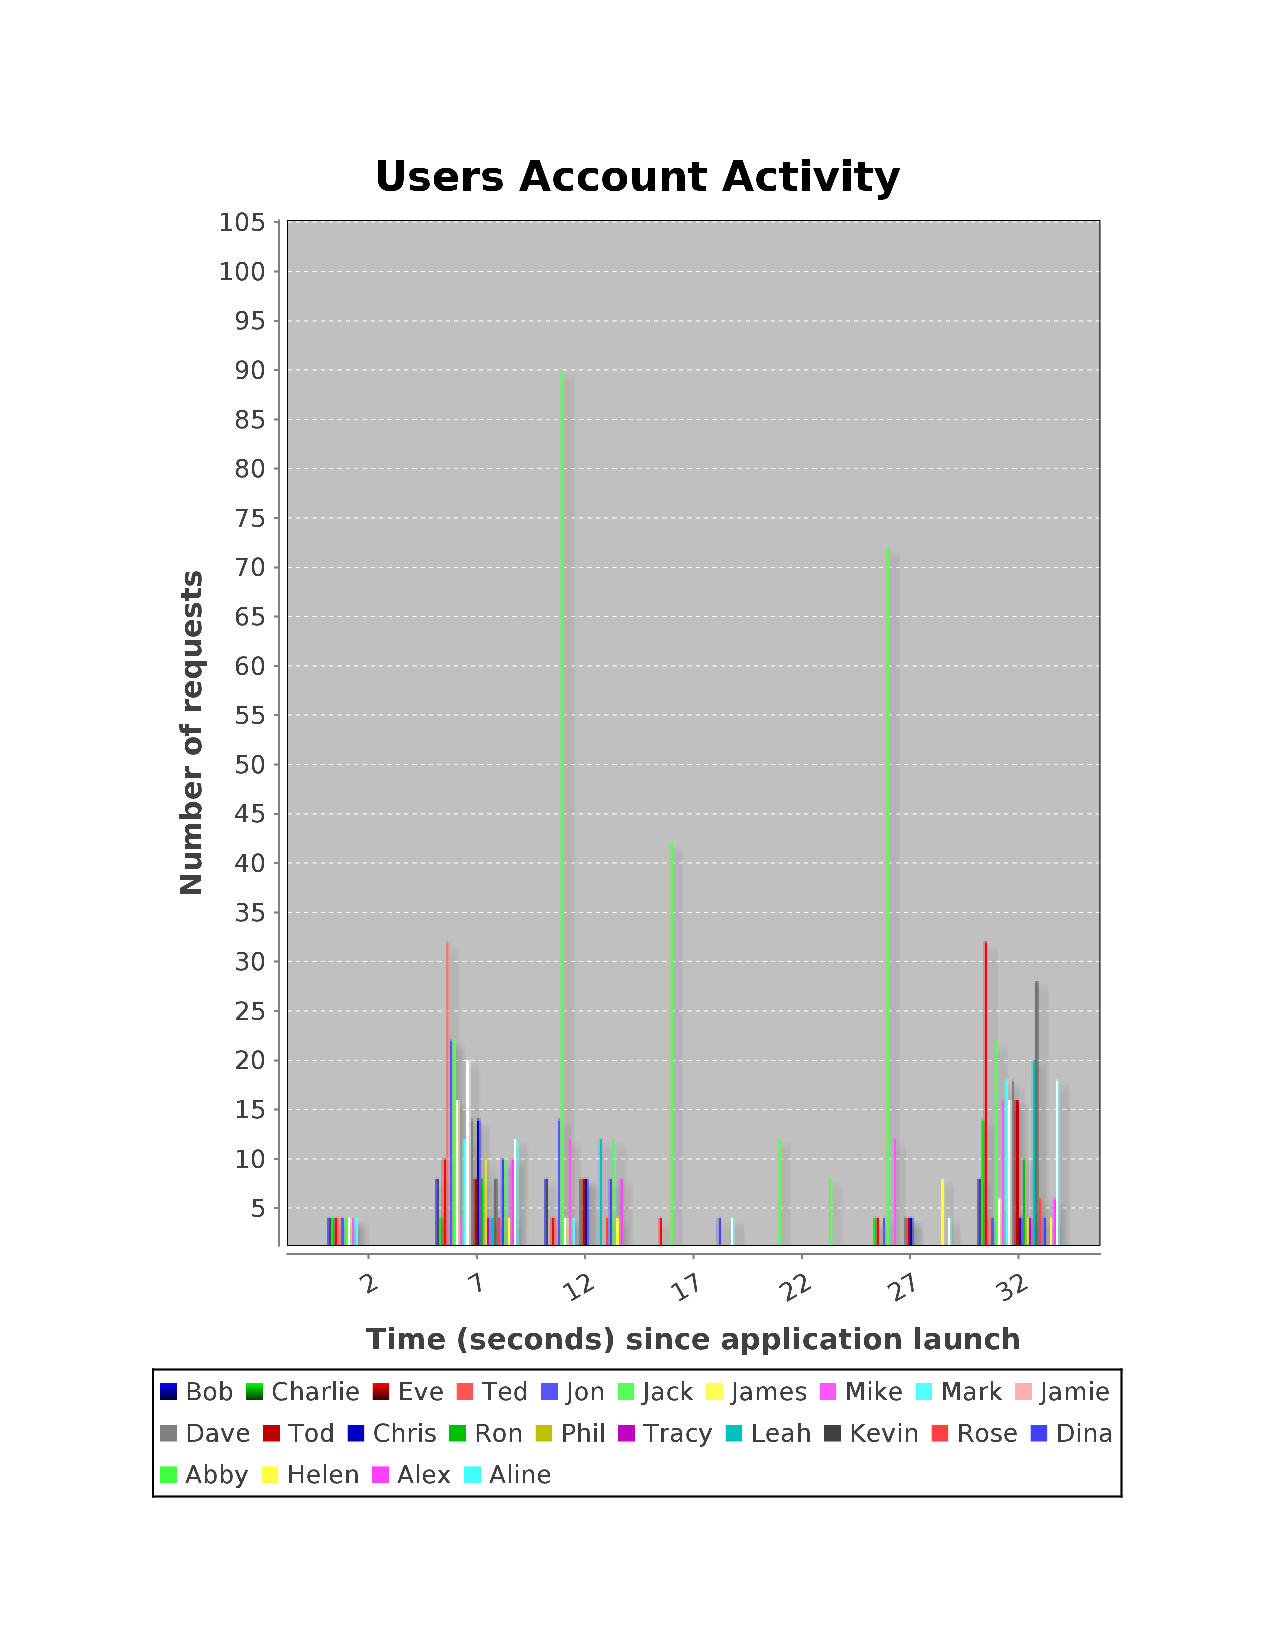
\includegraphics[width=\textwidth,height=\textheight,keepaspectratio]{figures/activity}
\caption{This graph shows the activity trend of each user. Notice that the activity for user Jack spikes in the graph at multiple places, this could be the result of an attacker accessing his account and issuing many requests to retreieve all of Jack's financial information in a short amount of time.}
\label{figure:activity}
\end{figure}
In this section we described how the data for Figure x can be extracted from the event log, as well as the possible uses of summarization for this scenario.

\section{Logging}

Aeolus provides a library that allows application developers to add their own application-specific events to the event log. These events are meant to help the developer attach semantic meaning to the event records in the log.

In order to gather the information necessary to produce the graph in figure x, we add application-specific event records to the event log for each different action the user takes.

For example, when a user signs up successfully with our application, we record their username, as well as the tag and principal associated with this user. This done using the following procedure:

\begin{lstlisting}[language=Java]
  AeolusLib.createEvent(``mint-signup'', username, principal, tag);
\end{lstlisting}

To obtain a table detailing the username, prinicpal, data tag and other sign-up information of all users, we use the following SQL query based on our application-specific events:\footnote{\emph{to\_array} is a procedure that turns a comma-delimited string into a PSQL array.}:

\begin{lstlisting}[language=SQL, deletendkeywords={TIMESTAMP}]
select to_array(app_arg)[0] as pid, to_array(app_arg)[1] as username, to_array(app_arg)[2] as tag, timestamp as signed_up, event_counter from events where op_name='mint-signup'
\end{lstlisting}

Table \ref{table:users-info} shows what such a view would look like, with some extra information about time swhen each user signed up. We can now use this table to extract more semantic information about the event log.

\begin{table}
\begin{verbatim}

 pid | username | tag  |        signed_up        | event_counter 
-----+----------+------+-------------------------+---------------
   6 | wissam   | [4]  | 2012-06-13 21:56:36.207 |           131
   9 | david    | [7]  | 2012-06-13 21:56:36.207 |           445
  12 | dan      | [10] | 2012-06-13 21:56:37.338 |           793
  13 | Bob      | [11] | 2012-06-13 21:56:37.338 |          1148
  14 | Charlie  | [12] | 2012-06-13 21:56:37.338 |          1211
  15 | Eve      | [13] | 2012-06-13 21:56:37.338 |          1274
  16 | Ted      | [14] | 2012-06-13 21:56:37.338 |          1337
  17 | Jon      | [15] | 2012-06-13 21:56:37.338 |          1400
  18 | Jack     | [16] | 2012-06-13 21:56:37.338 |          1463
  19 | James    | [17] | 2012-06-13 21:56:37.338 |          1526
  20 | Mike     | [18] | 2012-06-13 21:56:37.338 |          1589
  21 | Mark     | [19] | 2012-06-13 21:56:37.338 |          1652
  22 | Jamie    | [20] | 2012-06-13 21:56:38.578 |          1715
  23 | Dave     | [21] | 2012-06-13 21:56:38.578 |          1778
  24 | Tod      | [22] | 2012-06-13 21:56:38.578 |          1841
  25 | Chris    | [23] | 2012-06-13 21:56:38.578 |          1904
  26 | Ron      | [24] | 2012-06-13 21:56:38.578 |          1967
  27 | Phil     | [25] | 2012-06-13 21:56:38.578 |          2030
  28 | Tracy    | [26] | 2012-06-13 21:56:38.578 |          2093
  29 | Leah     | [27] | 2012-06-13 21:56:38.578 |          2156
  30 | Kevin    | [28] | 2012-06-13 21:56:38.578 |          2219
  31 | Rose     | [29] | 2012-06-13 21:56:38.578 |          2282
  32 | Dina     | [30] | 2012-06-13 21:56:38.578 |          2345
  33 | Abby     | [31] | 2012-06-13 21:56:38.578 |          2408
  34 | Helen    | [32] | 2012-06-13 21:56:38.578 |          2471
  35 | Alex     | [33] | 2012-06-13 21:56:38.578 |          2534
  36 | Aline    | [34] | 2012-06-13 21:56:38.578 |          2597

\end{verbatim}
\caption*{Users Table}
\caption{This is a table detailing the information of users signing up during a simulated run of the Mint application. The \emph{pid} column denotes the user's principal, the \emph{username} column denotes the user's username, the \emph{tag} column denotes the user's data tag, the \emph{signed\_up} column denotes the time at which the sign up event was logged to the system, and the \emph{event\_counter} column denotes the unique event\_counter number of the sign up event. }
\label{table:users-info}
\end{table}

For example, we can obtain the information necessary to create the graph in figure y using this query:

\begin{lstlisting}[language=SQL, deletendkeywords={TIMESTAMP}, label=query:accesses]
select e.count, users.username, e.to_timestamp as timestamp from (select count(*), tags_modified, (to_timestamp(((extract (epoch from events.timestamp)/5)::int)*5)) from events tags_modified in (select tag from users) group by (to_timestamp(((extract (epoch from events.timestamp)/5)::int)*5)), tags_modified) as e inner join users on e.tags_modified=users.tag
\end{lstlisting}

Table \ref{table:activity} shows a sample result of this query. This query provides us with a count of how many user requests caused a label modification that involved a user data tag for every 5-second period of time since the application launch, the information necessary to construct the graph in figure y.

\begin{table}
\begin{quote}
\begin{verbatim}
 count | username |       timestamp        
-------+----------+------------------------
    22 | Jack     | 2012-06-13 21:56:40-04
     4 | Jack     | 2012-06-13 21:56:35-04
    42 | Jack     | 2012-06-13 21:56:50-04
    72 | Jack     | 2012-06-13 21:57:00-04
    90 | Jack     | 2012-06-13 21:56:45-04
    12 | Jack     | 2012-06-13 21:56:55-04
    22 | Jack     | 2012-06-13 21:57:05-04
\end{verbatim}
\end{quote}
\caption*{Account activity for user \emph{Jack}}
\caption{This table shows a sample result of the \emph{accesses} view (for simplicity we only show the result for the user Jack). It details the number of user RPC requests causing a label manipulation involving a user data tag for every 5-second period since the application launched. The \emph{count} denotes such number. The \emph{username} column denotes the user who's data tag is in question. The \emph{timestamp} column denotes the start of the 5-second period.}
\label{table:activity}
\end{table}

\section{Summarization}

Creating summaries could prove to be very useful in auditing the Mint application. For example, if we store the \emph{count} in Figure \ref{table:activity} per user session.

In the next chapter, we present a system that allows us to summarize our log and extract the same information from the summary events, and we explain how to reach the same auditing information relying mostly on summary events.
